\documentclass[11pt,openany]{article}

\input{algebra-preamble}
\usepackage{commath}
\usepackage{caption}
%Tikzpicture
\usepackage{tikz}
\usepackage{tikz-3dplot}
\usepackage{tikz-cd}
\usetikzlibrary{
	3d, % For 3D drawing
	angles,
	arrows,
	arrows.meta,
	backgrounds,
	bending,
	calc,
	decorations.pathmorphing,
	decorations.pathreplacing,
	decorations.markings,
	fit,
	matrix,
	patterns,
	patterns.meta,
	positioning,
	quotes,
	shadows,
	shapes,
	shapes.geometric
}
\input{../preamble/tcolorbox}

\newcommand{\arrowboth}[1][]{\arrow[#1, bend left=15, myarrow]\arrow[bend left=15, myarrow, from=#1]}
\newcommand{\topology}{\mathcal{T}}

\setstretch{1.25}
\begin{document}
	\pagenumbering{arabic}
	\begin{center}
		\huge\textbf{Topology for Polynomial Rings}\\
		\vspace{0.5em}
		%	\Large\quad{대수학의 아름다움 서브-스터디}\\
		\vspace{0.5em}
		\normalsize{\today}\\
	\end{center}
	
\defbox[Topological Space]{
\textbf{Topological Space} is a set \( X \) with a collection \( \mathcal{T} \subseteq 2^X \) is a topological space if \( \mathcal{T} \) satisfies the following:
\begin{enumerate}
	\item \( \emptyset \in \mathcal{T} \) and \( X \in \mathcal{T} \) (inclusion of the empty set and the entire space).
	\item \( \mathcal{T} \) is closed under arbitrary unions, i.e., if \( \{ U_\alpha \}_{\alpha \in A} \subseteq \mathcal{T} \), then \( \bigcup_{\alpha \in A} U_\alpha \in \mathcal{T} \).
	\item \( \mathcal{T} \) is closed under finite intersections, i.e., if \( U_1, U_2, \ldots, U_n \in \mathcal{T} \), then \( \bigcap_{i=1}^n U_i \in \mathcal{T} \).
\end{enumerate}}
\begin{remark}
\ \begin{itemize}
	\item $\set{\emptyset, X}\subseteq\mathcal{T}$
	\item $\set{U_\alpha}_{\alpha\in A}\subseteq\topology\implies\bigcup_{\alpha\in A}U_\alpha\in\topology$
	\item $\set{U_i}_{i=1}^n\subseteq\topology\implies\bigcap_{i=1}^nU_i\in\topology$
\end{itemize}
\end{remark}

\defbox[Zero Set of Polynomials]{
Let \( X \) be a set and let \( \mathbb{K} \) be a field (such as \( \mathbb{R} \) or \( \mathbb{C} \)). Consider the ring of polynomials \( \mathbb{K}[x_1, x_2, \dots, x_n] \) in \( n \) variables with coefficients in \( \mathbb{K} \). For a polynomial \( f \in \mathbb{K}[x_1, x_2, \dots, x_n] \), the zero set of \( f:X\to\mathbb{K} \) is defined as:
\[
Z(f) = \{ \mathbf{x} = (x_1, x_2, \dots, x_n) \in X \mid f(\mathbf{x}) = 0 \}\subseteq X.
\]
More generally, for a collection of polynomials \( \{ f_\alpha \}_{\alpha \in A} \subseteq \mathbb{K}[x_1, x_2, \dots, x_n] \), the zero set of this collection is defined as:
\begin{align*}
	Z(\{ f_\alpha \}_{\alpha \in A}) &= \left\{ \mathbf{x} \in X \mid f_\alpha(\mathbf{x}) = 0 \text{ for all } \alpha \in A \right\} \\
	&=\bigcap_{\alpha \in A} \left\{ \mathbf{x} \in X \mid f_\alpha(\mathbf{x}) = 0 \right\} \\
	&=\bigcap_{\alpha \in A} Z(f_\alpha).
\end{align*}}

\probox[The Zero Set of Simultaneous Equations forms a Topology]{
Let \[
\mathcal{T} = \{ Z(f) \mid f \in \mathbb{K}[x_1, x_2, \dots, x_n] \}\subseteq 2^X \]
be the collection of zero sets of polynomials in \( \mathbb{K}[x_1, x_2, \dots, x_n] \). 
Then \( \mathcal{T} \) forms the collection of closed sets for a topology on \( X \).
}
\begin{proof}
	
To show that \( \mathcal{T} \) forms a topology, we must verify that \( \mathcal{T} \) satisfies the following conditions:

\begin{enumerate}
	\item \( X \in \mathcal{T} \) and \( \emptyset \in \mathcal{T} \).
	\item \( \mathcal{T} \) is closed under arbitrary intersections.
	\item \( \mathcal{T} \) is closed under finite unions.
\end{enumerate}

\subsubsection*{1. \( X \in \mathcal{T} \) and \( \emptyset \in \mathcal{T} \)}
\begin{itemize}
	\item[-] \textbf{\( X \in \mathcal{T} \)}: Consider the constant polynomial \( f(\mathbf{x}) = 0 \) for all \( \mathbf{x} \in X \). The zero set of \( f \) is: \[
	Z(f) = \{ \mathbf{x} \in X \mid f(\mathbf{x}) = 0 \} = X.
	\]
	Thus, \( X \in \mathcal{T} \).
	\item[-] \textbf{\( \emptyset \in \mathcal{T} \)}: Consider the constant polynomial \( g(\mathbf{x}) = 1 \) for all \( \mathbf{x} \in X \). The zero set of \( g \) is: \[
	Z(g) = \{ \mathbf{x} \in X \mid g(\mathbf{x}) = 0 \} = \emptyset.
	\]
	Thus, \( \emptyset \in \mathcal{T} \).
\end{itemize}

\subsubsection*{2. \( \mathcal{T} \) is Closed Under Arbitrary Intersections}
\begin{itemize}
	\item[-] Let \( \{ Z(f_\alpha) \}_{\alpha \in A} \) be a collection of zero sets where \( f_\alpha \in \mathbb{K}[x_1, x_2, \dots, x_n] \) for each \( \alpha \in A \).
	\item[-] Consider the intersection of these zero sets:
	\[
	\bigcap_{\alpha \in A} Z(f_\alpha) = \bigcap_{\alpha \in A} \{ \mathbf{x} \in X \mid f_\alpha(\mathbf{x}) = 0 \}.
	\]
	\item[-]  This can be rewritten as:
	\[
	\bigcap_{\alpha \in A} Z(f_\alpha) = \{ \mathbf{x} \in X \mid f_\alpha(\mathbf{x}) = 0 \text{ for all } \alpha \in A \}.
	\]
	\item[-] Define a new function \( g: X \to \mathbb{K} \) by:
	\[
	g(\mathbf{x}) = \sum_{\alpha \in A} f_\alpha(\mathbf{x})^2.
	\]
	Since \( f_\alpha(\mathbf{x})^2 \geq 0 \) for each \( \alpha \in A \), \( g(\mathbf{x}) = 0 \) if and only if \( f_\alpha(\mathbf{x}) = 0 \) for all \( \alpha \in A \).
	\item[-] Therefore, the intersection \( \bigcap_{\alpha \in A} Z(f_\alpha) \) is exactly \( Z(g) \), which is in \( \mathcal{T} \). Thus, \( \mathcal{T} \) is closed under arbitrary intersections.
\end{itemize}

\subsubsection*{3. \( \mathcal{T} \) is Closed Under Finite Unions}
\begin{itemize}
	\item[-] Consider two zero sets \( Z(f_1) \) and \( Z(f_2) \), where \( f_1, f_2 \in \mathbb{K}[x_1, x_2, \dots, x_n] \).
	\item[-] The union of these zero sets is:
	\[
	Z(f_1) \cup Z(f_2) = \{ \mathbf{x} \in X \mid f_1(\mathbf{x}) = 0 \text{ or } f_2(\mathbf{x}) = 0 \}.
	\]
	\item[-] Define a new function \( h: X \to \mathbb{K} \) by:
	\[
	h(\mathbf{x}) = f_1(\mathbf{x}) \cdot f_2(\mathbf{x}).
	\]
	\item[-] The zero set \( Z(h) \) is given by:
	\[
	Z(h) = \{ \mathbf{x} \in X \mid h(\mathbf{x}) = 0 \} = \{ \mathbf{x} \in X \mid f_1(\mathbf{x}) \cdot f_2(\mathbf{x}) = 0 \}.
	\]
	This is exactly the union \( Z(f_1) \cup Z(f_2) \).
	\item[-] Therefore, \( Z(f_1) \cup Z(f_2) = Z(h) \in \mathcal{T} \), showing that \( \mathcal{T} \) is closed under finite unions.
\end{itemize}
\end{proof}
\newpage

\section*{Proof that Maximal Ideal \( \implies \) Prime Ideal \( \implies \) Radical Ideal}

\subsection*{1. Maximal Ideal \( \implies \) Prime Ideal}

\textbf{Definitions:}
\begin{itemize}
	\item \textbf{Maximal Ideal:} An ideal \( M \) in a ring \( R \) is \textbf{maximal} if:
	\[
	M \subsetneq R \text{ and } \nexists I \text{ such that } M \subsetneq I \subsetneq R.
	\]
	
	\item \textbf{Prime Ideal:} An ideal \( P \) in a ring \( R \) is \textbf{prime} if:
	\[
	P \subsetneq R \text{ and } \forall a, b \in R, \; ab \in P \Rightarrow a \in P \text{ or } b \in P.
	\]
\end{itemize}

\textbf{Proof:} Let \( M \) be a maximal ideal in \( R \). We need to show that \( M \) is a prime ideal.

\begin{enumerate}
	\item \( M \) is proper: Since \( M \) is maximal, by definition, \( M \subsetneq R \).
	
	\item Prime condition: Suppose \( ab \in M \) for some \( a, b \in R \). Consider the ideal \( (M, a) \) generated by \( M \) and \( a \):
	\[
	(M, a) = \{ m + ra \mid m \in M, r \in R \}.
	\]
	Since \( M \) is maximal, there are two possibilities:
	\[
	(M, a) = M \quad \text{or} \quad (M, a) = R.
	\]
	\begin{itemize}
		\item If \( (M, a) = M \), then \( a \in M \).
		\item If \( (M, a) = R \), then there exist \( m \in M \) and \( r \in R \) such that:
		\[
		1 = m + ra.
		\]
		Multiplying both sides by \( b \), we get:
		\[
		b = mb + rab.
		\]
		Since \( mb \in M \) and \( ab \in M \) (because \( M \) is an ideal), it follows that \( b \in M \).
	\end{itemize}
\end{enumerate}

Hence, \( ab \in M \) implies \( a \in M \) or \( b \in M \), so \( M \) is a prime ideal.

\[
M \text{ maximal} \implies M \text{ prime}.
\]

\subsection*{2. Prime Ideal \( \implies \) Radical Ideal}

\textbf{Definitions:}
\begin{itemize}
	\item \textbf{Radical Ideal:} An ideal \( I \) in a ring \( R \) is \textbf{radical} if:
	\[
	\forall a \in R, \; a^n \in I \text{ for some } n \geq 1 \Rightarrow a \in I.
	\]
\end{itemize}

\textbf{Proof:} Let \( P \) be a prime ideal in \( R \). We need to show that \( P \) is also a radical ideal.

\begin{enumerate}
	\item \( P \) is proper: Since \( P \) is prime, \( P \subsetneq R \).
	
	\item Radical condition: Suppose \( a^n \in P \) for some \( n \geq 1 \). We need to show that \( a \in P \).
	
	\begin{itemize}
		\item Consider \( a^n \in P \). Since \( P \) is prime, the definition of a prime ideal implies:
		\[
		\text{If } a^n \in P, \text{ then } a \in P \text{ or } a^{n-1} \in P.
		\]
		\item If \( a \in P \), we are done.
		\item If \( a^{n-1} \in P \), apply the same argument to \( a^{n-1} \):
		\[
		\text{If } a^{n-1} \in P, \text{ then } a \in P \text{ or } a^{n-2} \in P.
		\]
		\item Repeating this process, we eventually conclude \( a \in P \).
	\end{itemize}
\end{enumerate}

Thus, \( P \) is a radical ideal.

\[
P \text{ prime} \implies P \text{ radical}.
\]

\subsection*{Conclusion}
By combining the results:

\[
\text{Maximal Ideal} \implies \text{Prime Ideal} \implies \text{Radical Ideal}.
\]

This completes the proof.

\newpage
\begin{itemize}
	\item $\C[x]=\set{\sum_{i=0}^{n}a_ix^i:a_i\in\C, n\in\Z_{\geq 0}}$
	\item $\C=\set{\alpha:\alpha\in\C}$
	\item Note that $\C\subseteq\C[x]$ since $\C=\set{\alpha:\alpha\in\C}=\set{0x^n+0x^{n-1}+\cdots+\alpha x^0:\alpha\in\C}$
	\item Consider \[
	\fullfunction{\phi_\alpha}{\C[x]}{\C}{f}{f(\alpha)}
	\] and 
	\item Consider $f(x)\in\C[x]$ s.t. \[
	\fullfunction{f}{\C}{\C}{\alpha}{f(\alpha)}
	\]
	\item By the first isomorphism theorem, we have $\C[x]/\gen{x-\alpha}\simeq\C$
	\item $\gen{x-\alpha}=\set{(x-\alpha)f(x):f(x)\in\C[x]}\subseteq\C[x]$
	\item $\C[x]/\gen{x-\alpha}$;
	\begin{itemize}
		\item $p(x)=(x-\alpha)q(x)+r(x)=(x-\alpha)q(x)+r$
		\item $\C[x]/\gen{x-\alpha}=\set{r+\gen{x-\alpha}:r\in\C}$
	\end{itemize}
\end{itemize}

\adjustbox{scale=.9}{\setstretch{1.5}
\begin{tabular}{|l||c|c|} \hline
	\textbf{Mapping} & $\fullfunction{\psi_p}{\Z}{\Z_p}{n}{n\bmod p=\psi_p(n)}$ & $\fullfunction{\phi_a}{\C[x]}{\C}{f(x)}{f(a)=\phi_a(f(x))}$ \\ \hline\hline
	Additive Homo. & $\psi_p(a+b):=(a+b)\bmod p$ & $\phi_a(f+g):=f(a)+g(a)$ \\ \hline
	Multiplicative Homo. & $\psi_p(ab):=(ab)\bmod p$ & $\phi_a(fg):=f(a)g(a)$ \\ \hline
	Kernel & $\ker(\psi_p)=p\Z$ & $\ker(\phi_a)=(x-a)\C[x]$ \\ \hline
	Image & $\Z_p$ & $\C$ \\ \hline
	Ideal & $p\Z=\gen{p}$ & $(x-a)\C[x]=\gen{x-a}$ \\ \hline
	Prime Ideal & $\gen{p}$ is prime & $\gen{x-a}$ is prime \\ \hline
	Maximal Ideal & $\gen{p}$ is maximal & $\gen{x-a}$ is maximal \\ \hline
	Isomorphism & $\Z_p\simeq \Z/p\Z$ & $\C\simeq \C[x]/\gen{x-a}$ \\ \hline
	Element of Domain & $\fullfunction{n}{arg2}{arg3}{arg4}{arg5}$ & $\fullfunction{f}{\set{\gen{x-\alpha}:\alpha\in\C}}{\coprod_{\alpha}\C[x]/\gen{x-\alpha}}{\gen{x-\alpha}}{arg5}$ \\ \hline
\end{tabular}}

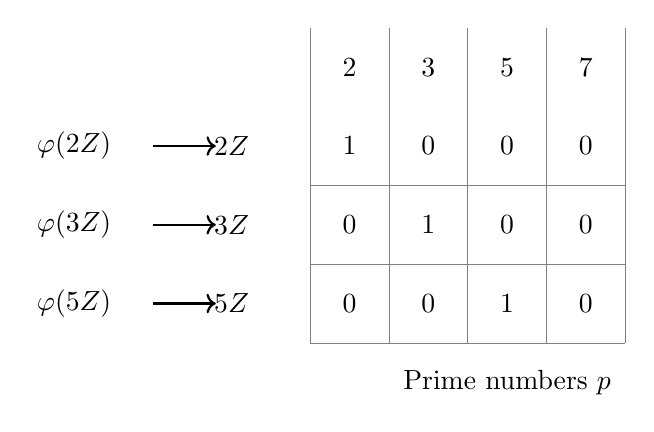
\begin{tikzpicture}[scale=1]
	
	% Draw the grid for primes
	\foreach \x in {0, 1, 2, 3, 4} {
		\draw[gray, very thin] (\x, 0) -- (\x, 4);
	}
	\foreach \y in {0, 1, 2} {
		\draw[gray, very thin] (0, \y) -- (4, \y);
	}
	
	% Labels for primes at the top
	\node at (0.5, 3.5) {2};
	\node at (1.5, 3.5) {3};
	\node at (2.5, 3.5) {5};
	\node at (3.5, 3.5) {7};
	
	% Labels for pZ on the left
	\node at (-1, 2.5) {$2\mathbb{Z}$};
	\node at (-1, 1.5) {$3\mathbb{Z}$};
	\node at (-1, 0.5) {$5\mathbb{Z}$};
	
	% Entries for pZ=2Z
	\node at (0.5, 2.5) {1}; % 1 mod 2 (for p = 2)
	\node at (1.5, 2.5) {0}; % 0 mod 3
	\node at (2.5, 2.5) {0}; % 0 mod 5
	\node at (3.5, 2.5) {0}; % 0 mod 7
	
	% Entries for pZ=3Z
	\node at (0.5, 1.5) {0}; % 0 mod 2
	\node at (1.5, 1.5) {1}; % 1 mod 3 (for p = 3)
	\node at (2.5, 1.5) {0}; % 0 mod 5
	\node at (3.5, 1.5) {0}; % 0 mod 7
	
	% Entries for pZ=5Z
	\node at (0.5, 0.5) {0}; % 0 mod 2
	\node at (1.5, 0.5) {0}; % 0 mod 3
	\node at (2.5, 0.5) {1}; % 1 mod 5 (for p = 5)
	\node at (3.5, 0.5) {0}; % 0 mod 7
	
	% Label for prime numbers
	\node at (2.5, -0.5) {Prime numbers $p$};
	
	% Arrow and description
	\draw[->, thick] (-2, 2.5) -- (-1.2, 2.5);
	\draw[->, thick] (-2, 1.5) -- (-1.2, 1.5);
	\draw[->, thick] (-2, 0.5) -- (-1.2, 0.5);
	
	\node at (-3, 2.5) {$\varphi(2\mathbb{Z})$};
	\node at (-3, 1.5) {$\varphi(3\mathbb{Z})$};
	\node at (-3, 0.5) {$\varphi(5\mathbb{Z})$};
	
\end{tikzpicture}

\end{document}
